
\documentclass[10pt,letterpaper,unboxed,cm]{article}
\usepackage[margin=1in]{geometry}
\usepackage{graphicx}
\usepackage{enumerate}

\newcommand{\st}{~\mid~}
\newcommand{\ind}{$~~~$}
\usepackage{xcolor}

\graphicspath{ {.././images} }

\begin{document}


\hfill{CSE 101 Spring 2024}
\hfill{Homework 3}
\hfill{Due: Wednesday 4/24 at 11:59pm}

\begin{enumerate}



\item
You are given a schedule for $n$ buses in the city. The schedule is given to you as a 2-dimensional array $B$ of dimensions $n\times k$. Each bus has $k$ stops and each entry of the array is an ordered pair $B[i,j] = (S_{i,j},t_{i,j})$  which means that the $j^{th}$ stop that bus $i$ makes is at station $S_{i,j}$ at time $t_{i,j}$ (measured in minutes counted from the beginning of the day.) Each row is ordered by times (i.e., $t_{i,1}<t_{i,2}<\dots <t_{i,k}$. 

You can transfer from bus $a$ to bus $b$ at stop $X$ if there exists entries $B[a,j] = (X,t_{a,j})$ and $B[b,j'] = (X,t_{b,j'})$ and $t_{a,j} < t_{b,j'}$.

\begin{enumerate}
\item
Given bus stations $X$ and $Y$ and a starting time $T$, design an algorithm that returns the earliest time you can reach station $Y$ from station $X$ starting any time after time $T$ using a sequence of transfers.
\item
Given bus stations $X$ and $Y$ and a starting time $T$, design an algorithm that returns the fewest number of transfers necessary to reach station $Y$ from station $X$ starting any time after time $T$ using a sequence of transfers.
\end{enumerate}





\item
For some non-negative integer $d$, we say that a $d$-regular graph is an undirected graph such that each vertex has a degree of $d$.

Suppose you are given access to a \emph{connected} $d$-regular graph $G=(V,E)$ and two vertices $s\in V$, $t\in V$. You wish to find the shortest path from $s$ to $t$. (We can assume that the graph is very large and that we want to avoid having to look at the entire graph. So, for any vertex, you can look at its list of neighbors without having to look at the entire graph.)


We can alter BFS so that it takes both $s$ and $t$ as inputs and when we reach $t$, we can stop so that we don't have to continue to explore unnecessary vertices.


\begin{quote}
\texttt{BFS2}$(G,s,t)$:
\begin{enumerate}[(1)]
\item
\texttt{for all} $u\in V$:
\item
\ind \texttt{dist}$(u) = \infty$
\item
\texttt{dist}$(s) = 0$
\item
$Q = [s]$
\item
\texttt{while} $Q$ \texttt{is not empty}:
\item
\ind $u = $ \texttt{eject}$(Q)$
\item
\ind \texttt{for all edges} $(u,v) \in E$:
\item
\ind \ind \texttt{if dist}$(v) = \infty$:
\item
\ind\ind\ind \texttt{inject}$(Q,v)$
\item
\ind\ind\ind \texttt{dist}$(v) = $ \texttt{dist}$(u)+1$
\item
\ind\ind\ind \texttt{if} $v == t$:
\item
\ind\ind\ind\ind \texttt{break loop}
\end{enumerate}
\end{quote}

(Notice that \texttt{BFS2} is almost identical to \texttt{BFS} except for lines 11 and 12.)

\begin{enumerate}
\item
\begin{enumerate}
\item
Give an argument about why \texttt{BFS2} will correctly assign \emph{dist}$(t)$ to the length of the shortest path from $s$ to $t$.

(3 points)



\item
Assuming that $\ell$ is the length of the shortest path from $s$ to $t$, what is the worst-case runtime of \texttt{BFS2} in terms of $d$ and $\ell$? (your answer should be in big-$O$ notation in terms of $d$ and $\ell$.)

(4 points)

(Note: You can use the fact that for every possible distance $i=1...L$, at some point in BFS, the queue will contain exactly all of the vertices that are distance $i$ away from $s$.)


\end{enumerate}

\item
Design an algorithm that finds the shortest path from $s$ to $t$ in $G$ that runs in time $O(d^{\ell/2})$.
\begin{enumerate}
\item
High-level algorithm description (No correctness proof necessary.) (4 points)


\item
Runtime analysis. (4 points)



\end{enumerate}
\end{enumerate}

\item
\emph{[The purpose of this problem is to show that Dijkstra's algorithm could be exponential time if run on a graph with negative edge weights.]}

For all integers $n\geq 0$, consider the graph $H(n)$ pictured below:

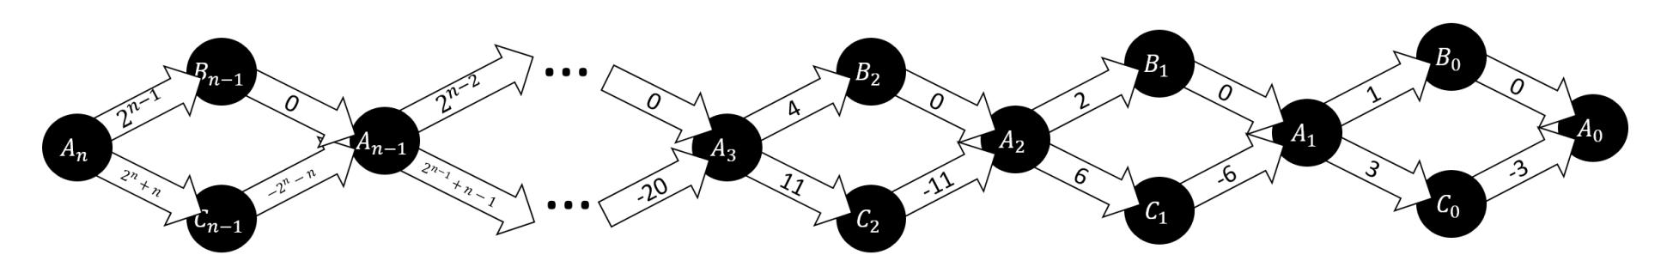
\includegraphics[scale=0.4]{Dijkstra_negative}

That is, $A_0$ has no outgoing neighbors and the adjacency list for each other vertex is:

\begin{itemize}
\item
$A_k: (B_{k-1},2^{k-1}),(C_{k-1},2^k + k)$
\item
$B_k: (A_{k},0)$
\item
$C_k: (A_{k}, -2^k - k)$ 
\end{itemize}

\begin{enumerate}
\item
Let $maxdist(v)$ be the maximum dist value that $dist(v)$ is set to (besides $\infty$) after running Dijkstra's on $H(n)$ starting at $A_n$.

Prove by induction that $maxdist(v)\leq 2^n+n$ for all $v\in H(n)$.

\item
Prove by induction that after running Dijkstra's on $H(n)$, starting at $A_n$, the vertex $A_0$ has been ejected from the priority queue $2^n$ times. (You can use the previous part.)

\item
Give a lower bound for the runtime of Dijkstra's on this graph in $\Omega$ notation in terms of the number of vertices $N$.
\end{enumerate}

\item
Suppose Dijkstra's algorithm is run on the following graph, starting at node $A$.
\begin{enumerate}
\item
Draw a table showing the intermediate distance values of all the nodes at each iteration of the algorithm. (5 points)
\item
Draw the shortest path tree.
(5 points)

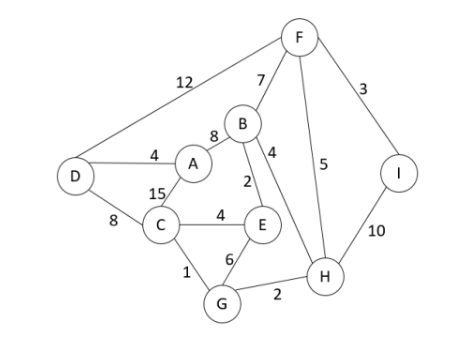
\includegraphics[scale=0.4]{Dijkstras}
\end{enumerate}

\end{enumerate}


\end{document}